\chapter{Software and Hardware Infrastructure}
\label{chapter:SHI}
In this chapter, we will describe the software and hardware
infrastructure used in this thesis. In Section~\ref{sec:ros} we will introduce the
Robot Operating System, and the Personal Robot 2 (PR2) robot will be presented in Section
~\ref{sec:pr2}. This is followed by the introduction of OpenCV library.

\section{The Robot Operating System (ROS)}
\label{sec:ros}
% provides libraries and tools to help
% software developers create robot applications. It provides hardware
% abstraction, device drivers, libraries, visualizers, message-passing,
% package management, and more.
ROS is an open-source, meta-operating framework for robot software
development. ROS was originally developed in 2007 by Stanford Artificial Intelligence Laboratory in support of the Stanford AI Robot~\cite{quigley2007stair}. Like an ordinary operating system, it consists of  robot
hardware resources management, low-level device control, implementation
of commonly-used functionality, inter-processes communication (\acronym{IPC}{inter-processes communication}), and package
management. ROS is based on a peer-to-peer network architecture where
processing takes place in nodes that may receive, post, control, state
messages. There are several different styles of communication, including synchronous RPC-style communication over services, asynchronous
streaming of data over topics, and storage of data on a Parameter
Server.
Moreover, ROS provides tools and libraries for obtaining, building, writing, and
running code across multiple computers.

ROS is composed of core and federated package components. The former one is a fundamental library as described
above and the latter one is a suit of user contributed packages which
are organized into sets called \textit{stacks}. The stacks include
many application areas, such as  perception, object identification,
segmentation and recognition, face recognition, motion tracking ,
stereopsis stereo vision, control, planning, grasping and so on. ROS has been ported to many robots and boards.

The goal of ROS is "to support code reuse in robotics research and
development"~\cite{rosintroduction}.  it is designed to enable easily
share and collaborate among developers. Moreover, ROS has many
features, such as compact framework, language independence, easy
testing and scalability.

ROS currently run on on Unix-like operating systems towards which the library is
geared. Currently Ubuntu Linux is greatly supported. Moreover, the core
ROS system and its tools and libraries are regularly released as ROS
Distributions~\cite{rosintroduction} under the terms of the BSD
license. More detail about ROS can be found here:\url{http://www.ros.org/wiki/}.
\section{The PR2 Robot}
\label{sec:pr2}
Personal Robot 2 (Fig.~\ref{fig:pr2}) is a personal robotics research and development
platform.  It is developed by Willow Garage.  PR2 has two 7-DOF arms and a mobile
base, and its size  is similar to a human. Its sensors system consists of a 5
mega-pixel camera, a tilting laser range finder, and an inertial
measurement unit. The "texture projector" on PR2 can project a pattern
on the environment to create 3D information captured by the
cameras. PR2 is equipped with 16 CPU cores with 48 Gigabytes of
RAM. Its battery system consists of 16 laptop batteries. PR2 is
controlled with ROS system as described in Section~\ref{sec:ros} which
consists of a series of libraries for perception, navigation and
manipulation.
The experiments of this thesis were partly generated on PR2 as
depicted in Fig.~\ref{fig:pr2}.

\begin{figure}[htbp]
  \centering
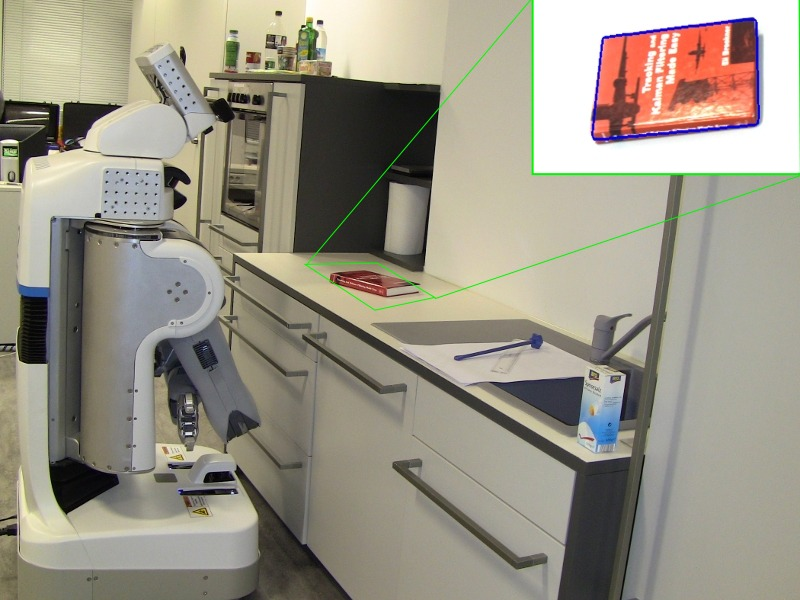
\includegraphics[width=\linewidth]{images/pr2.jpg}
  \caption[The PR2 robot]{The PR2 robot located in central CoTeSys
    Robotic Lab at Technische Universit\"at M\"unchen.}
  \label{fig:pr2}
\end{figure}

\section{OpenCV Library}
\label{sec:opencv}

Open Source Computer Vision Library (OpenCV)~\cite{opencv} is a library of
programming functions mainly aimed at real time computer vision. It is
originally developed by Intel and now maintained by Willow Garage. It
is free for both academic and commercial usage and released  under the
open source BSD license. The library is cross-platform, which supports
Windows, Linux and MacOX,  in the latest version 2.2, the Android
system is supported.

OpenCV is originally written in C but now full C++ and Python
interfaces are provided. The library is widely used in the field of
computer vision, such as Human-Computer Interaction (\acronym{HCI}{Human-Computer Interaction}); Object
Identification, Segmentation and Recognition; Face Recognition;
Gesture Recognition; Motion Tracking, Ego Motion, Motion
Understanding, Stereo and Multi-Camera
Calibration and Depth Computation, Mobile Robotics (e.g. Android
system).

\begin{figure}[htbp]
  \centering
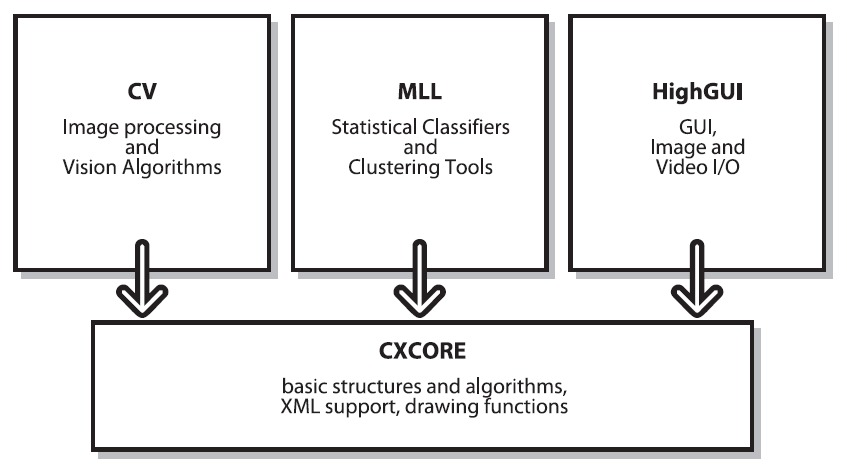
\includegraphics[width=\linewidth]{images/bsopencv.jpg}
  \caption[The basic structure of the OpenCV library]{The basic
    structure of the OpenCV library~\cite{bradski2008learning}}
  \label{fig:bsopencv}
\end{figure}

Currently, OpenCV consists of following main components~\cite{bradski2008learning}.
\begin{itemize}
\item \textbf{core}: The basic data structures and content
\item \textbf{imgproc}: Image processing and vision algorithms
\item \textbf{mll}: Machine learning library, including statistical classifiers and clustering tools.
\item \textbf{highgui}: Graphic user interface and Input/Output
  routines for image and video
\item \textbf{calib3d}: Camera calibration and 3d reconstruction
\item \textbf{features2d}: Feature detection and descriptor extraction
\item \textbf{flann}: Clustering and search in multi-dimensional spaces
\item \textbf{haartraining}: Rapid object detection with a cascade of boosted classifiers based on Haar-like features
\item \textbf{objdetect}: Algorithms used to detect objects
\item \textbf{gpu}: A set of classes and functions to utilize GPU computational capabilities
\item \textbf{python}: Libraries to provide Python interface
\item \textbf{video}: Video analysis
\end{itemize}

The B-spline and CCD algorithm in this thesis is implemented using the
OpenCV library.
